\begin{figure}[htb]
\centering
\textbf{Roof types for construction types of two typologies}\\
\vspace{-0.6cm} 

  \begin{tabular}{p{0.5\textwidth} p{0.5\textwidth}}

\hspace{-1.4cm}
% Created by tikzDevice version 0.8.1 on 2015-03-03 13:54:10
% !TEX encoding = UTF-8 Unicode
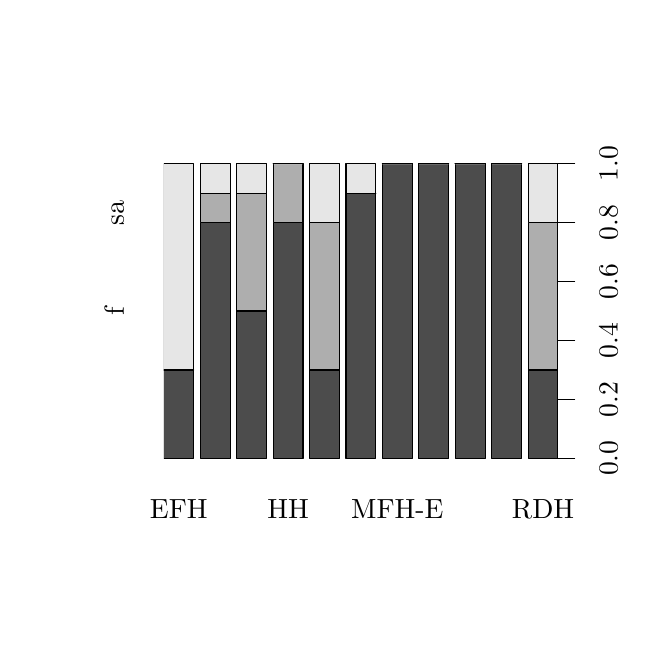
\begin{tikzpicture}[x=1pt,y=1pt]
\definecolor{fillColor}{RGB}{255,255,255}
\path[use as bounding box,fill=fillColor,fill opacity=0.00] (0,0) rectangle (216.81,216.81);
\begin{scope}
\path[clip] (  0.00,  0.00) rectangle (216.81,216.81);
\definecolor{drawColor}{RGB}{0,0,0}

\end{scope}
\begin{scope}
\path[clip] ( 49.20, 61.20) rectangle (191.61,167.61);
\definecolor{drawColor}{RGB}{0,0,0}
\definecolor{fillColor}{gray}{0.30}

\path[draw=drawColor,line width= 0.4pt,line join=round,line cap=round,fill=fillColor] ( 49.20, 61.20) rectangle ( 59.99, 93.12);
\definecolor{fillColor}{RGB}{174,174,174}

\path[draw=drawColor,line width= 0.4pt,line join=round,line cap=round,fill=fillColor] ( 49.20, 93.12) rectangle ( 59.99, 93.12);
\definecolor{fillColor}{RGB}{230,230,230}

\path[draw=drawColor,line width= 0.4pt,line join=round,line cap=round,fill=fillColor] ( 49.20, 93.12) rectangle ( 59.99,167.61);
\definecolor{fillColor}{gray}{0.30}

\path[draw=drawColor,line width= 0.4pt,line join=round,line cap=round,fill=fillColor] ( 62.36, 61.20) rectangle ( 73.15,146.33);
\definecolor{fillColor}{RGB}{174,174,174}

\path[draw=drawColor,line width= 0.4pt,line join=round,line cap=round,fill=fillColor] ( 62.36,146.33) rectangle ( 73.15,156.97);
\definecolor{fillColor}{RGB}{230,230,230}

\path[draw=drawColor,line width= 0.4pt,line join=round,line cap=round,fill=fillColor] ( 62.36,156.97) rectangle ( 73.15,167.61);
\definecolor{fillColor}{gray}{0.30}

\path[draw=drawColor,line width= 0.4pt,line join=round,line cap=round,fill=fillColor] ( 75.52, 61.20) rectangle ( 86.31,114.41);
\definecolor{fillColor}{RGB}{174,174,174}

\path[draw=drawColor,line width= 0.4pt,line join=round,line cap=round,fill=fillColor] ( 75.52,114.41) rectangle ( 86.31,156.97);
\definecolor{fillColor}{RGB}{230,230,230}

\path[draw=drawColor,line width= 0.4pt,line join=round,line cap=round,fill=fillColor] ( 75.52,156.97) rectangle ( 86.31,167.61);
\definecolor{fillColor}{gray}{0.30}

\path[draw=drawColor,line width= 0.4pt,line join=round,line cap=round,fill=fillColor] ( 88.69, 61.20) rectangle ( 99.48,146.33);
\definecolor{fillColor}{RGB}{174,174,174}

\path[draw=drawColor,line width= 0.4pt,line join=round,line cap=round,fill=fillColor] ( 88.69,146.33) rectangle ( 99.48,167.61);
\definecolor{fillColor}{RGB}{230,230,230}

\path[draw=drawColor,line width= 0.4pt,line join=round,line cap=round,fill=fillColor] ( 88.69,167.61) rectangle ( 99.48,167.61);
\definecolor{fillColor}{gray}{0.30}

\path[draw=drawColor,line width= 0.4pt,line join=round,line cap=round,fill=fillColor] (101.85, 61.20) rectangle (112.64, 93.12);
\definecolor{fillColor}{RGB}{174,174,174}

\path[draw=drawColor,line width= 0.4pt,line join=round,line cap=round,fill=fillColor] (101.85, 93.12) rectangle (112.64,146.33);
\definecolor{fillColor}{RGB}{230,230,230}

\path[draw=drawColor,line width= 0.4pt,line join=round,line cap=round,fill=fillColor] (101.85,146.33) rectangle (112.64,167.61);
\definecolor{fillColor}{gray}{0.30}

\path[draw=drawColor,line width= 0.4pt,line join=round,line cap=round,fill=fillColor] (115.01, 61.20) rectangle (125.80,156.97);
\definecolor{fillColor}{RGB}{174,174,174}

\path[draw=drawColor,line width= 0.4pt,line join=round,line cap=round,fill=fillColor] (115.01,156.97) rectangle (125.80,156.97);
\definecolor{fillColor}{RGB}{230,230,230}

\path[draw=drawColor,line width= 0.4pt,line join=round,line cap=round,fill=fillColor] (115.01,156.97) rectangle (125.80,167.61);
\definecolor{fillColor}{gray}{0.30}

\path[draw=drawColor,line width= 0.4pt,line join=round,line cap=round,fill=fillColor] (128.17, 61.20) rectangle (138.96,167.61);
\definecolor{fillColor}{RGB}{174,174,174}

\path[draw=drawColor,line width= 0.4pt,line join=round,line cap=round,fill=fillColor] (128.17,167.61) rectangle (138.96,167.61);
\definecolor{fillColor}{RGB}{230,230,230}

\path[draw=drawColor,line width= 0.4pt,line join=round,line cap=round,fill=fillColor] (128.17,167.61) rectangle (138.96,167.61);
\definecolor{fillColor}{gray}{0.30}

\path[draw=drawColor,line width= 0.4pt,line join=round,line cap=round,fill=fillColor] (141.33, 61.20) rectangle (152.12,167.61);
\definecolor{fillColor}{RGB}{174,174,174}

\path[draw=drawColor,line width= 0.4pt,line join=round,line cap=round,fill=fillColor] (141.33,167.61) rectangle (152.12,167.61);
\definecolor{fillColor}{RGB}{230,230,230}

\path[draw=drawColor,line width= 0.4pt,line join=round,line cap=round,fill=fillColor] (141.33,167.61) rectangle (152.12,167.61);
\definecolor{fillColor}{gray}{0.30}

\path[draw=drawColor,line width= 0.4pt,line join=round,line cap=round,fill=fillColor] (154.50, 61.20) rectangle (165.29,167.61);
\definecolor{fillColor}{RGB}{174,174,174}

\path[draw=drawColor,line width= 0.4pt,line join=round,line cap=round,fill=fillColor] (154.50,167.61) rectangle (165.29,167.61);
\definecolor{fillColor}{RGB}{230,230,230}

\path[draw=drawColor,line width= 0.4pt,line join=round,line cap=round,fill=fillColor] (154.50,167.61) rectangle (165.29,167.61);
\definecolor{fillColor}{gray}{0.30}

\path[draw=drawColor,line width= 0.4pt,line join=round,line cap=round,fill=fillColor] (167.66, 61.20) rectangle (178.45,167.61);
\definecolor{fillColor}{RGB}{174,174,174}

\path[draw=drawColor,line width= 0.4pt,line join=round,line cap=round,fill=fillColor] (167.66,167.61) rectangle (178.45,167.61);
\definecolor{fillColor}{RGB}{230,230,230}

\path[draw=drawColor,line width= 0.4pt,line join=round,line cap=round,fill=fillColor] (167.66,167.61) rectangle (178.45,167.61);
\definecolor{fillColor}{gray}{0.30}

\path[draw=drawColor,line width= 0.4pt,line join=round,line cap=round,fill=fillColor] (180.82, 61.20) rectangle (191.61, 93.12);
\definecolor{fillColor}{RGB}{174,174,174}

\path[draw=drawColor,line width= 0.4pt,line join=round,line cap=round,fill=fillColor] (180.82, 93.12) rectangle (191.61,146.33);
\definecolor{fillColor}{RGB}{230,230,230}

\path[draw=drawColor,line width= 0.4pt,line join=round,line cap=round,fill=fillColor] (180.82,146.33) rectangle (191.61,167.61);
\end{scope}
\begin{scope}
\path[clip] (  0.00,  0.00) rectangle (216.81,216.81);
\definecolor{drawColor}{RGB}{0,0,0}

\node[text=drawColor,anchor=base,inner sep=0pt, outer sep=0pt, scale=  1.00] at ( 54.59, 39.60) {EFH};

\node[text=drawColor,anchor=base,inner sep=0pt, outer sep=0pt, scale=  1.00] at ( 94.08, 39.60) {HH};

\node[text=drawColor,anchor=base,inner sep=0pt, outer sep=0pt, scale=  1.00] at (133.57, 39.60) {MFH-E};

\node[text=drawColor,anchor=base,inner sep=0pt, outer sep=0pt, scale=  1.00] at (186.22, 39.60) {RDH};

\node[text=drawColor,rotate= 90.00,anchor=base,inner sep=0pt, outer sep=0pt, scale=  1.00] at ( 34.80,114.41) {f};

\node[text=drawColor,rotate= 90.00,anchor=base,inner sep=0pt, outer sep=0pt, scale=  1.00] at ( 34.80,149.88) {sa};

\path[draw=drawColor,line width= 0.4pt,line join=round,line cap=round] (191.61, 61.20) -- (191.61,167.61);

\path[draw=drawColor,line width= 0.4pt,line join=round,line cap=round] (191.61, 61.20) -- (197.61, 61.20);

\path[draw=drawColor,line width= 0.4pt,line join=round,line cap=round] (191.61, 82.48) -- (197.61, 82.48);

\path[draw=drawColor,line width= 0.4pt,line join=round,line cap=round] (191.61,103.76) -- (197.61,103.76);

\path[draw=drawColor,line width= 0.4pt,line join=round,line cap=round] (191.61,125.05) -- (197.61,125.05);

\path[draw=drawColor,line width= 0.4pt,line join=round,line cap=round] (191.61,146.33) -- (197.61,146.33);

\path[draw=drawColor,line width= 0.4pt,line join=round,line cap=round] (191.61,167.61) -- (197.61,167.61);

\node[text=drawColor,rotate= 90.00,anchor=base,inner sep=0pt, outer sep=0pt, scale=  1.00] at (213.21, 61.20) {0.0};

\node[text=drawColor,rotate= 90.00,anchor=base,inner sep=0pt, outer sep=0pt, scale=  1.00] at (213.21, 82.48) {0.2};

\node[text=drawColor,rotate= 90.00,anchor=base,inner sep=0pt, outer sep=0pt, scale=  1.00] at (213.21,103.76) {0.4};

\node[text=drawColor,rotate= 90.00,anchor=base,inner sep=0pt, outer sep=0pt, scale=  1.00] at (213.21,125.05) {0.6};

\node[text=drawColor,rotate= 90.00,anchor=base,inner sep=0pt, outer sep=0pt, scale=  1.00] at (213.21,146.33) {0.8};

\node[text=drawColor,rotate= 90.00,anchor=base,inner sep=0pt, outer sep=0pt, scale=  1.00] at (213.21,167.61) {1.0};
\end{scope}
<<<<<<< HEAD
\end{tikzpicture}
=======
\end{tikzpicture}
>>>>>>> 36a956db0f2ffb15b4b8091da9293464a1b25a0c
&
\hspace{-1.4cm}
% Created by tikzDevice version 0.8.1 on 2015-03-03 13:54:12
% !TEX encoding = UTF-8 Unicode
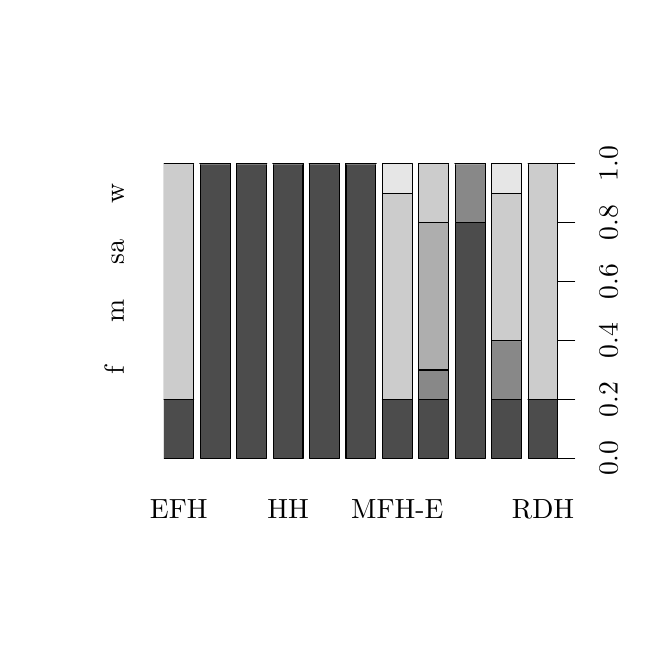
\begin{tikzpicture}[x=1pt,y=1pt]
\definecolor{fillColor}{RGB}{255,255,255}
\path[use as bounding box,fill=fillColor,fill opacity=0.00] (0,0) rectangle (216.81,216.81);
\begin{scope}
\path[clip] (  0.00,  0.00) rectangle (216.81,216.81);
\definecolor{drawColor}{RGB}{0,0,0}

\end{scope}
\begin{scope}
\path[clip] ( 49.20, 61.20) rectangle (191.61,167.61);
\definecolor{drawColor}{RGB}{0,0,0}
\definecolor{fillColor}{gray}{0.30}

\path[draw=drawColor,line width= 0.4pt,line join=round,line cap=round,fill=fillColor] ( 49.20, 61.20) rectangle ( 59.99, 82.48);
\definecolor{fillColor}{RGB}{136,136,136}

\path[draw=drawColor,line width= 0.4pt,line join=round,line cap=round,fill=fillColor] ( 49.20, 82.48) rectangle ( 59.99, 82.48);
\definecolor{fillColor}{RGB}{174,174,174}

\path[draw=drawColor,line width= 0.4pt,line join=round,line cap=round,fill=fillColor] ( 49.20, 82.48) rectangle ( 59.99, 82.48);
\definecolor{fillColor}{gray}{0.80}

\path[draw=drawColor,line width= 0.4pt,line join=round,line cap=round,fill=fillColor] ( 49.20, 82.48) rectangle ( 59.99,167.61);
\definecolor{fillColor}{RGB}{230,230,230}

\path[draw=drawColor,line width= 0.4pt,line join=round,line cap=round,fill=fillColor] ( 49.20,167.61) rectangle ( 59.99,167.61);
\definecolor{fillColor}{gray}{0.30}

\path[draw=drawColor,line width= 0.4pt,line join=round,line cap=round,fill=fillColor] ( 62.36, 61.20) rectangle ( 73.15,167.61);
\definecolor{fillColor}{RGB}{136,136,136}

\path[draw=drawColor,line width= 0.4pt,line join=round,line cap=round,fill=fillColor] ( 62.36,167.61) rectangle ( 73.15,167.61);
\definecolor{fillColor}{RGB}{174,174,174}

\path[draw=drawColor,line width= 0.4pt,line join=round,line cap=round,fill=fillColor] ( 62.36,167.61) rectangle ( 73.15,167.61);
\definecolor{fillColor}{gray}{0.80}

\path[draw=drawColor,line width= 0.4pt,line join=round,line cap=round,fill=fillColor] ( 62.36,167.61) rectangle ( 73.15,167.61);
\definecolor{fillColor}{RGB}{230,230,230}

\path[draw=drawColor,line width= 0.4pt,line join=round,line cap=round,fill=fillColor] ( 62.36,167.61) rectangle ( 73.15,167.61);
\definecolor{fillColor}{gray}{0.30}

\path[draw=drawColor,line width= 0.4pt,line join=round,line cap=round,fill=fillColor] ( 75.52, 61.20) rectangle ( 86.31,167.61);
\definecolor{fillColor}{RGB}{136,136,136}

\path[draw=drawColor,line width= 0.4pt,line join=round,line cap=round,fill=fillColor] ( 75.52,167.61) rectangle ( 86.31,167.61);
\definecolor{fillColor}{RGB}{174,174,174}

\path[draw=drawColor,line width= 0.4pt,line join=round,line cap=round,fill=fillColor] ( 75.52,167.61) rectangle ( 86.31,167.61);
\definecolor{fillColor}{gray}{0.80}

\path[draw=drawColor,line width= 0.4pt,line join=round,line cap=round,fill=fillColor] ( 75.52,167.61) rectangle ( 86.31,167.61);
\definecolor{fillColor}{RGB}{230,230,230}

\path[draw=drawColor,line width= 0.4pt,line join=round,line cap=round,fill=fillColor] ( 75.52,167.61) rectangle ( 86.31,167.61);
\definecolor{fillColor}{gray}{0.30}

\path[draw=drawColor,line width= 0.4pt,line join=round,line cap=round,fill=fillColor] ( 88.69, 61.20) rectangle ( 99.48,167.61);
\definecolor{fillColor}{RGB}{136,136,136}

\path[draw=drawColor,line width= 0.4pt,line join=round,line cap=round,fill=fillColor] ( 88.69,167.61) rectangle ( 99.48,167.61);
\definecolor{fillColor}{RGB}{174,174,174}

\path[draw=drawColor,line width= 0.4pt,line join=round,line cap=round,fill=fillColor] ( 88.69,167.61) rectangle ( 99.48,167.61);
\definecolor{fillColor}{gray}{0.80}

\path[draw=drawColor,line width= 0.4pt,line join=round,line cap=round,fill=fillColor] ( 88.69,167.61) rectangle ( 99.48,167.61);
\definecolor{fillColor}{RGB}{230,230,230}

\path[draw=drawColor,line width= 0.4pt,line join=round,line cap=round,fill=fillColor] ( 88.69,167.61) rectangle ( 99.48,167.61);
\definecolor{fillColor}{gray}{0.30}

\path[draw=drawColor,line width= 0.4pt,line join=round,line cap=round,fill=fillColor] (101.85, 61.20) rectangle (112.64,167.61);
\definecolor{fillColor}{RGB}{136,136,136}

\path[draw=drawColor,line width= 0.4pt,line join=round,line cap=round,fill=fillColor] (101.85,167.61) rectangle (112.64,167.61);
\definecolor{fillColor}{RGB}{174,174,174}

\path[draw=drawColor,line width= 0.4pt,line join=round,line cap=round,fill=fillColor] (101.85,167.61) rectangle (112.64,167.61);
\definecolor{fillColor}{gray}{0.80}

\path[draw=drawColor,line width= 0.4pt,line join=round,line cap=round,fill=fillColor] (101.85,167.61) rectangle (112.64,167.61);
\definecolor{fillColor}{RGB}{230,230,230}

\path[draw=drawColor,line width= 0.4pt,line join=round,line cap=round,fill=fillColor] (101.85,167.61) rectangle (112.64,167.61);
\definecolor{fillColor}{gray}{0.30}

\path[draw=drawColor,line width= 0.4pt,line join=round,line cap=round,fill=fillColor] (115.01, 61.20) rectangle (125.80,167.61);
\definecolor{fillColor}{RGB}{136,136,136}

\path[draw=drawColor,line width= 0.4pt,line join=round,line cap=round,fill=fillColor] (115.01,167.61) rectangle (125.80,167.61);
\definecolor{fillColor}{RGB}{174,174,174}

\path[draw=drawColor,line width= 0.4pt,line join=round,line cap=round,fill=fillColor] (115.01,167.61) rectangle (125.80,167.61);
\definecolor{fillColor}{gray}{0.80}

\path[draw=drawColor,line width= 0.4pt,line join=round,line cap=round,fill=fillColor] (115.01,167.61) rectangle (125.80,167.61);
\definecolor{fillColor}{RGB}{230,230,230}

\path[draw=drawColor,line width= 0.4pt,line join=round,line cap=round,fill=fillColor] (115.01,167.61) rectangle (125.80,167.61);
\definecolor{fillColor}{gray}{0.30}

\path[draw=drawColor,line width= 0.4pt,line join=round,line cap=round,fill=fillColor] (128.17, 61.20) rectangle (138.96, 82.48);
\definecolor{fillColor}{RGB}{136,136,136}

\path[draw=drawColor,line width= 0.4pt,line join=round,line cap=round,fill=fillColor] (128.17, 82.48) rectangle (138.96, 82.48);
\definecolor{fillColor}{RGB}{174,174,174}

\path[draw=drawColor,line width= 0.4pt,line join=round,line cap=round,fill=fillColor] (128.17, 82.48) rectangle (138.96, 82.48);
\definecolor{fillColor}{gray}{0.80}

\path[draw=drawColor,line width= 0.4pt,line join=round,line cap=round,fill=fillColor] (128.17, 82.48) rectangle (138.96,156.97);
\definecolor{fillColor}{RGB}{230,230,230}

\path[draw=drawColor,line width= 0.4pt,line join=round,line cap=round,fill=fillColor] (128.17,156.97) rectangle (138.96,167.61);
\definecolor{fillColor}{gray}{0.30}

\path[draw=drawColor,line width= 0.4pt,line join=round,line cap=round,fill=fillColor] (141.33, 61.20) rectangle (152.12, 82.48);
\definecolor{fillColor}{RGB}{136,136,136}

\path[draw=drawColor,line width= 0.4pt,line join=round,line cap=round,fill=fillColor] (141.33, 82.48) rectangle (152.12, 93.12);
\definecolor{fillColor}{RGB}{174,174,174}

\path[draw=drawColor,line width= 0.4pt,line join=round,line cap=round,fill=fillColor] (141.33, 93.12) rectangle (152.12,146.33);
\definecolor{fillColor}{gray}{0.80}

\path[draw=drawColor,line width= 0.4pt,line join=round,line cap=round,fill=fillColor] (141.33,146.33) rectangle (152.12,167.61);
\definecolor{fillColor}{RGB}{230,230,230}

\path[draw=drawColor,line width= 0.4pt,line join=round,line cap=round,fill=fillColor] (141.33,167.61) rectangle (152.12,167.61);
\definecolor{fillColor}{gray}{0.30}

\path[draw=drawColor,line width= 0.4pt,line join=round,line cap=round,fill=fillColor] (154.50, 61.20) rectangle (165.29,146.33);
\definecolor{fillColor}{RGB}{136,136,136}

\path[draw=drawColor,line width= 0.4pt,line join=round,line cap=round,fill=fillColor] (154.50,146.33) rectangle (165.29,167.61);
\definecolor{fillColor}{RGB}{174,174,174}

\path[draw=drawColor,line width= 0.4pt,line join=round,line cap=round,fill=fillColor] (154.50,167.61) rectangle (165.29,167.61);
\definecolor{fillColor}{gray}{0.80}

\path[draw=drawColor,line width= 0.4pt,line join=round,line cap=round,fill=fillColor] (154.50,167.61) rectangle (165.29,167.61);
\definecolor{fillColor}{RGB}{230,230,230}

\path[draw=drawColor,line width= 0.4pt,line join=round,line cap=round,fill=fillColor] (154.50,167.61) rectangle (165.29,167.61);
\definecolor{fillColor}{gray}{0.30}

\path[draw=drawColor,line width= 0.4pt,line join=round,line cap=round,fill=fillColor] (167.66, 61.20) rectangle (178.45, 82.48);
\definecolor{fillColor}{RGB}{136,136,136}

\path[draw=drawColor,line width= 0.4pt,line join=round,line cap=round,fill=fillColor] (167.66, 82.48) rectangle (178.45,103.76);
\definecolor{fillColor}{RGB}{174,174,174}

\path[draw=drawColor,line width= 0.4pt,line join=round,line cap=round,fill=fillColor] (167.66,103.76) rectangle (178.45,103.76);
\definecolor{fillColor}{gray}{0.80}

\path[draw=drawColor,line width= 0.4pt,line join=round,line cap=round,fill=fillColor] (167.66,103.76) rectangle (178.45,156.97);
\definecolor{fillColor}{RGB}{230,230,230}

\path[draw=drawColor,line width= 0.4pt,line join=round,line cap=round,fill=fillColor] (167.66,156.97) rectangle (178.45,167.61);
\definecolor{fillColor}{gray}{0.30}

\path[draw=drawColor,line width= 0.4pt,line join=round,line cap=round,fill=fillColor] (180.82, 61.20) rectangle (191.61, 82.48);
\definecolor{fillColor}{RGB}{136,136,136}

\path[draw=drawColor,line width= 0.4pt,line join=round,line cap=round,fill=fillColor] (180.82, 82.48) rectangle (191.61, 82.48);
\definecolor{fillColor}{RGB}{174,174,174}

\path[draw=drawColor,line width= 0.4pt,line join=round,line cap=round,fill=fillColor] (180.82, 82.48) rectangle (191.61, 82.48);
\definecolor{fillColor}{gray}{0.80}

\path[draw=drawColor,line width= 0.4pt,line join=round,line cap=round,fill=fillColor] (180.82, 82.48) rectangle (191.61,167.61);
\definecolor{fillColor}{RGB}{230,230,230}

\path[draw=drawColor,line width= 0.4pt,line join=round,line cap=round,fill=fillColor] (180.82,167.61) rectangle (191.61,167.61);
\end{scope}
\begin{scope}
\path[clip] (  0.00,  0.00) rectangle (216.81,216.81);
\definecolor{drawColor}{RGB}{0,0,0}

\node[text=drawColor,anchor=base,inner sep=0pt, outer sep=0pt, scale=  1.00] at ( 54.59, 39.60) {EFH};

\node[text=drawColor,anchor=base,inner sep=0pt, outer sep=0pt, scale=  1.00] at ( 94.08, 39.60) {HH};

\node[text=drawColor,anchor=base,inner sep=0pt, outer sep=0pt, scale=  1.00] at (133.57, 39.60) {MFH-E};

\node[text=drawColor,anchor=base,inner sep=0pt, outer sep=0pt, scale=  1.00] at (186.22, 39.60) {RDH};

\node[text=drawColor,rotate= 90.00,anchor=base,inner sep=0pt, outer sep=0pt, scale=  1.00] at ( 34.80, 93.12) {f};

\node[text=drawColor,rotate= 90.00,anchor=base,inner sep=0pt, outer sep=0pt, scale=  1.00] at ( 34.80,114.41) {m};

\node[text=drawColor,rotate= 90.00,anchor=base,inner sep=0pt, outer sep=0pt, scale=  1.00] at ( 34.80,135.69) {sa};

\node[text=drawColor,rotate= 90.00,anchor=base,inner sep=0pt, outer sep=0pt, scale=  1.00] at ( 34.80,156.97) {w};

\path[draw=drawColor,line width= 0.4pt,line join=round,line cap=round] (191.61, 61.20) -- (191.61,167.61);

\path[draw=drawColor,line width= 0.4pt,line join=round,line cap=round] (191.61, 61.20) -- (197.61, 61.20);

\path[draw=drawColor,line width= 0.4pt,line join=round,line cap=round] (191.61, 82.48) -- (197.61, 82.48);

\path[draw=drawColor,line width= 0.4pt,line join=round,line cap=round] (191.61,103.76) -- (197.61,103.76);

\path[draw=drawColor,line width= 0.4pt,line join=round,line cap=round] (191.61,125.05) -- (197.61,125.05);

\path[draw=drawColor,line width= 0.4pt,line join=round,line cap=round] (191.61,146.33) -- (197.61,146.33);

\path[draw=drawColor,line width= 0.4pt,line join=round,line cap=round] (191.61,167.61) -- (197.61,167.61);

\node[text=drawColor,rotate= 90.00,anchor=base,inner sep=0pt, outer sep=0pt, scale=  1.00] at (213.21, 61.20) {0.0};

\node[text=drawColor,rotate= 90.00,anchor=base,inner sep=0pt, outer sep=0pt, scale=  1.00] at (213.21, 82.48) {0.2};

\node[text=drawColor,rotate= 90.00,anchor=base,inner sep=0pt, outer sep=0pt, scale=  1.00] at (213.21,103.76) {0.4};

\node[text=drawColor,rotate= 90.00,anchor=base,inner sep=0pt, outer sep=0pt, scale=  1.00] at (213.21,125.05) {0.6};

\node[text=drawColor,rotate= 90.00,anchor=base,inner sep=0pt, outer sep=0pt, scale=  1.00] at (213.21,146.33) {0.8};

\node[text=drawColor,rotate= 90.00,anchor=base,inner sep=0pt, outer sep=0pt, scale=  1.00] at (213.21,167.61) {1.0};
\end{scope}
<<<<<<< HEAD
\end{tikzpicture}
=======
\end{tikzpicture}
>>>>>>> 36a956db0f2ffb15b4b8091da9293464a1b25a0c
\\

  \end{tabular}

\vspace{-1.4cm}

\begin{flushright}
\footnotesize{data source:
\cite{Born.2003,Hermelink.2011}}
\end{flushright}	
	\caption[Different values for roof types of building typologies used in
	Germany.]{Different values for roof types of building typologies used in
	Germany.
	The building types are arrange construction type in alphabetical order along
	the X-axis.
	The Y-axis shows the roof types of the single typologies.
	EFH; EFH-b; GMH; HH; KMH; KMH-b; MFH-E; MFH-E; MFH-G; MFH-H; MFH-W; RDH.
	(sa) pitched roof, ``Satteldach'';
	(m) curg roof, ``Mansardendach'';
	(w) hip roof, ``Walmdach'';
	(f) flat roof, ``Flachdach'';
	(so) other, ``Sonstiges''.}
	\label{fig:DifTypRoof}
\end{figure}